
% VLDB template version of 2020-08-03 enhances the ACM template, version 1.7.0:
% https://www.acm.org/publications/proceedings-template
% The ACM Latex guide provides further information about the ACM template

% \documentclass[sigconf, nonacm, pdfa]{acmart}
\documentclass[sigconf, nonacm]{acmart}
\usepackage{algorithmic}
\usepackage{caption}
\usepackage[ruled,vlined]{algorithm2e}
\usepackage{booktabs}
% \usepackage[a-2b]{pdfx}
\usepackage{pifont}
\usepackage{fancyhdr} % 导入fancyhdr包
\pagestyle{fancy}
\usepackage{color}
\usepackage{soul, framed}
\usepackage{makecell}
\usepackage{xcolor}
\usepackage{colortbl}
\usepackage{amsmath}
\usepackage{tikz}
\usetikzlibrary{positioning,arrows.meta,shapes.geometric,fit}
\usepackage{graphicx}
\usepackage{textcomp}
\usepackage{xcolor,colortbl}
\usepackage{multirow}
\usepackage{bm,dsfont}
\usepackage{subfigure}
\usepackage{balance}
\usepackage{stmaryrd}
\usepackage{autobreak}
\usepackage{enumitem}
\usepackage{bbding}
\usepackage{pifont}
\usepackage{wasysym}
% \usepackage{amssymb}
% \usepackage{lineno}


\newtheorem{definition}{Definition}
\newtheorem{lemma}{Lemma}
\newtheorem{remark}{Remark}
\newtheorem{example}{Example}
\newtheorem{theorem}{Theorem}
% \newtheorem{proof}{Proof}
\newcommand{\tabincell}[2]{\begin{tabular}{@{}#1@{}}#2\end{tabular}}


%\newcommand{\netname}{\textit{BOLA}{\xspace}}
\newcommand{\framework}{\textit{MomentBound}}
\newcommand{\paircnt}{\textit{pair}}
\newcommand{\triplecnt}{\textit{triple}}
\newcommand{\pcnt}{\text{pc}}
\newcommand{\tcnt}{\text{tc}}


%% The following content must be adapted for the final version
% paper-specific
% \newcommand\vldbdoi{XX.XX/XXX.XX}

% TODO: replace placeholder VLDB block at camera-ready
\newcommand\vldbdoi{XX.XX/XXX.XX}
\newcommand\vldbpages{XXX-XXX}
% issue-specific
\newcommand\vldbvolume{XX}
\newcommand\vldbissue{X}
\newcommand\vldbyear{20XX}
% should be fine as it is
\newcommand\vldbauthors{\authors}
\newcommand\vldbtitle{\shorttitle} 
% leave empty if no availability url should be set
\newcommand\vldbavailabilityurl{https://github.com/guaiyoui/logic_bugs}
% whether page numbers should be shown or not, use 'plain' for review versions, 'empty' for camera ready
% \newcommand\vldbpagestyle{plain} 
\newcommand\vldbpagestyle{empty}
\fancyfoot[C]{\thepage}

\begin{document}
\title{MomentBound: Join-Size Bounds as Polynomial Certificates\\over Degree Fields}

\author{Jianwei Wang}
\affiliation{%
  \institution{University of New South Wales}
  }
\email{jianwei.wang1@unsw.edu.au}
\orcid{0009-0000-7887-4179}

% \authornote{Kai Wang is the corresponding author.}

\author{Kai Wang}
% \authornotemark[1]
\affiliation{%
  \institution{ACEM, Shanghai Jiao Tong University}
}
\email{w.kai@sjtu.edu.cn}
\orcid{0000-0002-3123-2184}

\author{Xuemin Lin}
\affiliation{%
 \institution{ACEM, Shanghai Jiao Tong University}
  }
\email{xuemin.lin@sjtu.edu.cn}
\orcid{0000-0003-2396-7225}

\author{Wenjie Zhang}
\affiliation{%
  \institution{University of New South Wales}
  }
\email{wenjie.zhang@unsw.edu.au}
\orcid{0000-0001-6572-2600}

\author{Ying Zhang}
% \authornote{Ying Zhang and Kai Wang are the joint corresponding authors.}
\affiliation{%
  \institution{Zhejiang Gongshang University}
  }
\email{ying.zhang@zjgsu.edu.cn}
\orcid{0000-0002-2674-1638}

% \author{Jianwei Wang$^{1}$ ~~ Kai Wang$^{2}$ ~~ Xuemin Lin$^{2}$~~Wenjie Zhang$^{1}$ ~~Ying Zhang$^{3}$}
% \affiliation{\normalsize{$^{1}${The University of New South Wales, Sydney, Australia}}\\
%  \normalsize{$^{2}${Antai College of Economics \& Management, Shanghai Jiao Tong University, Shanghai, China}} \\
%  \normalsize{$^{3}${Zhejiang Gongshang University, Hangzhou, China}}}
% \email{{jianwei.wang1, wenjie.zhang}@unsw.edu.au, {w.kai, xuemin.lin}@sjtu.edu.cn, ying.zhang@zjgsu.edu.cn}

\begin{abstract}
Pessimistic cardinality estimation computes a \emph{guaranteed} upper
bound on the output size of a query from precomputed statistics on the
base relations.  The state of the art, LpBound, feeds
$\ell_p$-norms of per-relation degree sequences into a polymatroid
linear program over entropic variables.  We observe that these
statistics are all \emph{univariate}: they record the multiset of
degrees but not their alignment across relations, while the join size
itself is an inner product of degree sequences.  We therefore propose
to treat join-size bounding as a \emph{moment problem on a degree
field}: every key of a join attribute carries a degree vector, the
true join size is its product moment, and every statistic is an
observed moment $\mu_\alpha = \sum_x d(x)^\alpha$.  A bound is then a
nonnegativity certificate --- a conic combination of observed
monomials dominating the product polynomial on a worst-case domain ---
computed by a small linear program whose dual is a worst-case
alignment of the degree field.  This yields a Lasserre-style
hierarchy in which $\ell_p$ norms are the level-1 (univariate)
moments and exact $k$-way join counts are the higher levels, and it
comes with exactness criteria: on star queries the bound collapses to
the truth at the highest observed order, and one level earlier under
key-collapse.  Instantiated inside the entropy LP, pair and triple
join counts tighten the state of the art by up to an order of
magnitude in geometric-mean q-error on the standard LpBound
benchmarks (JOB-light, JOB-join, JOB-range on IMDB; STATS; DBLP
subgraph matching), e.g.\ geomean $175\to 8.3$ on STATS, at a storage
cost of one scalar per connected atom subset, while preserving a
formal bound guarantee that we verify with LP-dual certificates on
every query.
\end{abstract}

\begin{CCSXML}
<ccs2012>
   <concept>
       <concept_id>10002951.10003227</concept_id>
       <concept_desc>Information systems~Information systems applications</concept_desc>
       <concept_significance>500</concept_significance>
       </concept>
 </ccs2012>
\end{CCSXML}

\maketitle

%%% do not modify the following VLDB block %%
%%% VLDB block start %%%
\pagestyle{\vldbpagestyle}
\begingroup\small\noindent\raggedright\textbf{PVLDB Reference Format:}\\
\vldbauthors. \vldbtitle. PVLDB, \vldbvolume(\vldbissue): \vldbpages, \vldbyear.\\
\href{https://doi.org/\vldbdoi}{doi:\vldbdoi}
\endgroup
\begingroup
\renewcommand\thefootnote{}\footnote{\noindent
This work is licensed under the Creative Commons BY-NC-ND 4.0 International License. Visit \url{https://creativecommons.org/licenses/by-nc-nd/4.0/} to view a copy of this license. For any use beyond those covered by this license, obtain permission by emailing \href{mailto:info@vldb.org}{info@vldb.org}. Copyright is held by the owner/author(s). Publication rights licensed to the VLDB Endowment. \\
\raggedright Proceedings of the VLDB Endowment, Vol. \vldbvolume, No. \vldbissue\ %
ISSN 2150-8097. \\
\href{https://doi.org/\vldbdoi}{doi:\vldbdoi} \\
}\addtocounter{footnote}{-1}\endgroup
%%% VLDB block end %%%

%%% do not modify the following VLDB block %%
%%% VLDB block start %%%
\ifdefempty{\vldbavailabilityurl}{}{
\vspace{.3cm}
\begingroup\small\noindent\raggedright\textbf{PVLDB Artifact Availability:}\\
The source code, data, and/or other artifacts have been made available at \url{https://github.com/guaiyoui/logic_bugs}.
\endgroup
}
%%% VLDB block end %%%

\section{Introduction}
\label{sec:Introduction}

\begin{table*}
\caption{Comparison among provable join-size bounds}
\centering \scalebox{0.9}{
\begin{tabular}
{@{}lccccc@{}}
\toprule[1.2pt]
Bound & \makecell[c]{Statistics}   & \makecell[c]{Cross-relation\\alignment?}    & \makecell[c]{Form}  & \makecell[c]{Storage\\per statistic} & \makecell[c]{Exact on\\stars?}          \\ \midrule
AGM~\cite{atserias2013size,atserias2008agm} & relation sizes $|R|$ & \XSolidBrush & edge-cover LP & $O(1)$ & \XSolidBrush \\
PCE~\cite{cai2019pessimistic} & sizes $+$ max degrees & \XSolidBrush & per-join rollup & $O(1)$ & \XSolidBrush \\
SafeBound~\cite{deeds2023safebound}/DSB~\cite{deeds2023degree} & (compressed) degree sequences & \XSolidBrush & functional approx. & $O(\text{segments})$ & \makecell[c]{Berge-acyclic\\only} \\
LpBound~\cite{zhang2025lpbound,abokhamis2024lp} & $\ell_p$-norms of degree seq. & \XSolidBrush & entropy LP & $O(|P|)$ & \XSolidBrush \\
CorrBound~\cite{mayer2026corrbound} & sketched inner products & \makecell[c]{\Checkmark\\(approximate)} & entropy LP & $O(\text{sketch})$ & \XSolidBrush \\
\midrule
\framework~(ours) & exact $k$-way join counts $=$ moments $\mu_\alpha$ & \makecell[c]{\Checkmark\\(exact)} & \makecell[c]{entropy LP $+$\\certificate LP} & $O(1)$ & \makecell[c]{\Checkmark\\(order $m$, or\\$m{-}1$ under\\key-collapse)} \\ \bottomrule
\end{tabular}}
\label{tab:intro_comparasion}
\end{table*}


Cardinality estimation (CE) --- predicting the output size of a query
without evaluating it --- remains, four decades on, the optimizer's
Achilles heel~\cite{leis2015howgood,han2021cardinality}.
Underestimates are the catastrophic failure mode: they steer the
optimizer toward plans designed for small data, causing intermediate
results to explode at runtime.  This observation has motivated a line
of work on \emph{pessimistic} cardinality estimation (PCE): compute a
\emph{provable upper bound} on the join size from statistics
precomputed on the base relations~\cite{cai2019pessimistic,
deeds2023degree,deeds2023safebound,abokhamis2024lp,zhang2025lpbound}.
A bound that is never violated doubles as a soundness oracle for any
estimator~\cite{stoian2026outofbounds}, and injected into an
optimizer it provably eliminates catastrophic
plans~\cite{zhang2025lpbound}.

The state of the art is LpBound~\cite{zhang2025lpbound,
abokhamis2024lp}.  Its statistics are $\ell_p$-norms of
\emph{degree sequences}: for a join attribute $X$ of relation $R$,
$\deg_R(X)$ is the multiset of value frequencies, and its norms
$\|\deg_R(X)\|_p$ feed a polymatroid linear program whose variables
are the joint entropies $h(U)$ of attribute subsets of the query
output.  Each statistic enters through a \emph{$q$-inequality}
$(1/p)h(U) + h(V\,|\,U) \le \log\|\deg_R(V\,|\,U)\|_p$ --- one
application of H\"older's inequality --- and the optimum
$2^{h(V)}$ upper-bounds $|Q|$.

\vspace{1mm}
\noindent\textbf{The blind spot: univariate statistics.}
Every statistic LpBound observes is a function of the \emph{multiset}
of degrees of one relation at a time.  But the size of a join is an
inner product: $|R\Join_X S| = \sum_x \deg_R(x)\cdot\deg_S(x)$, which
depends entirely on how the two sequences \emph{align} over the key
domain.  As a consequence, three databases can share every $\ell_p$
norm yet differ in join size by orders of magnitude:

\begin{center}\small
\begin{tabular}{l|c|c}
alignment & same degree multisets & $\sum_x a_x b_x$ \\ \hline
ranks aligned & $a{=}[8,4,2], b{=}[9,3,1]$ & $86$ \\
ranks reversed & $a{=}[8,4,2], b{=}[1,3,9]$ & $38$ \\
disjoint supports & $a{=}[8,4,2], b{=}[0,0,0]$ & $0$ \\
\end{tabular}
\end{center}

\noindent No univariate-statistic bound can separate these instances;
any tighter bound must observe \emph{joint} information across
relations.  The question is which joint statistic to buy, at what
storage cost, and with what formal guarantee.

\vspace{1mm}
\noindent\textbf{Our framework: bounds as polynomial certificates.}
We answer this question by re-founding the problem itself.  On a star
join $R_1\Join_X\cdots\Join_X R_m$, every key $x$ of the separator
$X$ carries a \emph{degree vector}
$d(x) = (d_1(x),\dots,d_m(x))\in\mathbf{N}^m$, and the join size is
the \emph{product moment} of this \emph{degree field}:
$|Q| = \sum_x \prod_i d_i(x)$.  Every statistic is an observed moment
$\mu_\alpha = \sum_x d(x)^\alpha$ --- including LpBound's, since
$\mu_{p\cdot e_i} = \|\deg_i\|_p^p$.  A bound is then nothing more
(and nothing less) than a \emph{nonnegativity certificate}: a conic
combination of observed monomials that dominates the product
polynomial pointwise, $\prod_i d_i \le \sum_\alpha c_\alpha d^\alpha$
on a worst-case domain $\Omega$.  AM--GM, Young, and H\"older's
inequalities are the closed-form points of this cone; the certificate
LP finds the best member adapted to the observed moments.  Its dual
is the \emph{alignment LP}: the largest product moment attainable by
redistributing the degree field subject to the observed moments ---
so a bound is literally a worst-case alignment, and the certificate
is its proof.

This single object reorganizes the design space:

\begin{itemize}[leftmargin=10pt,itemsep=1pt]
\item \emph{A hierarchy, not a statistic.}  Observing the moments
  $\{\alpha : |\alpha|_1\le k\}$ defines a monotone Lasserre-style
  hierarchy~\cite{lasserre2001} over the field: level 1 is the
  univariate $\ell_p$ statistics of LpBound; level 2 adds exact pair
  join counts $|R_i\Join R_j| = \mu_{e_i+e_j}$; level 3 adds triple
  counts; level $m$ is exact, since $\mu_{\mathbf{1}}$ \emph{is} the
  product moment.
\item \emph{Exactness criteria.}  We characterize when a level
  collapses to the truth: on star queries, always at order $m$, and
  at order $m{-}1$ under a \emph{key-collapse} condition (one atom is
  a key on the separator and covers the others' supports) --- both
  verified empirically on real data.
\item \emph{A computable gain predictor.}  The H\"older gap
  $\log\frac{\min\text{-conjugate}\prod\|d_i\|}{\langle d_i,d_j\rangle}$
  measures what the level-2 moment buys over level 1 per pair ---
  turning statistic selection into a principled problem.
\item \emph{A symmetric lower-bound wing.}  The same moment LP at its
  minimum is a provable \emph{lower} bound (cf.\
  xBound~\cite{stoian2026xbound}); we show where the polynomial cone
  fails there and identify the correct (hinge) basis.
\end{itemize}

\vspace{1mm}
\noindent\textbf{Instantiation and results.}
Practically, we instantiate the hierarchy inside the entropic LP:
each exact $k$-way join count yields a support constraint
$h(\cup_{i\in S}A_i) \le \log|\Join_{i\in S} R_i|$ --- the strongest
constraint obtainable from one scalar --- whose soundness is a
two-line support argument (no new inequality family is needed,
unlike~\cite{mayer2026corrbound}).  A reduced LP keeps the method
computable on queries with up to $23$ attributes, and LP duality
emits a machine-checkable proof certificate for every bound.

On the LpBound evaluation suite (JOB-light/JOB-join/JOB-range on
IMDB~\cite{leis2015howgood,leis2018query}, STATS on
StackOverflow~\cite{han2021cardinality}, DBLP dense subgraph
patterns), all with zero violations:
pair moments alone reach geomean q-error \textbf{4.97} (vs.\ 16.14)
on JOB-light, \textbf{5.05} (vs.\ 10.07) on JOB-join, and
\textbf{7.30} (vs.\ 111.0) on JOB-range; on STATS the pair arm
reaches 88.5 (vs.\ 175.3) and triples collapse it further to
\textbf{8.28} --- a $21\times$ geomean improvement, with 34\% of
queries estimated \emph{exactly}.  On DBLP the method provably ties
the baseline --- a predicted negative control where degree sequences
already determine the alignment.  The certificate LP reproduces the
entropy LP query-by-query on all 69 star queries of STATS
($\le$3\% geomean divergence), confirming that the two formulations
are views of one object.

\vspace{1mm}
\noindent\textbf{Contributions.}
\begin{itemize}[leftmargin=10pt,itemsep=1pt]
\item \textbf{Theory}: a self-contained formulation of join-size
  bounds as a moment problem on the degree field, with bounds as
  polynomial certificates and a dual alignment LP (\S\ref{sec:theory});
  a Lasserre-style hierarchy with exactness criteria (key-collapse
  lemma); and a lower-bound wing with its basis limitation.
\item \textbf{Method}: pair/triple join-count statistics as support
  constraints in the entropic LP, a reduced LP for scalability to
  23-attribute queries, and dual proof certificates
  (\S\ref{sec:method}).
\item \textbf{Evaluation}: the full LpBound suite with zero
  violations and up to $21\times$ geomean improvement, plus a
  certificate-vs-entropy cross-validation on 69 real star queries
  (\S\ref{sec:exp}).
\end{itemize}

\section{Preliminaries}
\label{sec:Preliminary}

\begin{table}[t]
\centering \small
\caption{Symbols and Descriptions}
\label{tab:symbol}
\begin{tabular}{|p{2.1cm}|p{5.7cm}|}
\hline
\cellcolor{lightgray}\textbf{Notation} & \cellcolor{lightgray}\textbf{Description} \\ \hline
$Q$, $R_i$, $A_i$ & conjunctive query, $i$-th atom, its attribute set \\ \hline
$V$, $n$ & all attributes of $Q$, $n = |V|$ \\ \hline
$\deg_R(V|U)$ & degree sequence: multiplicities of $V$-values over each $U$-value of $R$ \\ \hline
$\|d\|_p$ & $\ell_p$-norm $(\sum_x d_x^p)^{1/p}$ \\ \hline
$h(U)$ & joint entropy of attributes $U$ in a distribution \\ \hline
$d(x)$, $\mathcal{D}$ & degree vector of key $x$, and the degree field \\ \hline
$\mu_\alpha$ & observed moment $\sum_x d(x)^\alpha$ \\ \hline
$\Omega$ & worst-case dominance domain $\prod_i \mathrm{supp}(\deg_i)$ \\ \hline
$\mathcal{A}$ & moment set $\{\alpha\}$ that is observed \\ \hline
$UB(\mathcal{A})$, $LB(\mathcal{A})$ & certificate bound under moments $\mathcal{A}$ \\ \hline
\end{tabular}
\end{table}

\subsection{Problem Statement}

A \emph{conjunctive query} (CQ) has the form
\begin{equation}
Q(V) \;=\; R_1(A_1) \Join R_2(A_2) \Join \cdots \Join R_m(A_m),
\label{eq:cq}
\end{equation}
where each atom $R_i$ is a relation whose schema is $A_i \subseteq V$
and $\bigcup_i A_i = V$; selection predicates on individual atoms are
folded into the (filtered) relations.  We write $|Q|$ for the output
size under bag semantics (SQL \texttt{COUNT(*)}).

\begin{definition}[Pessimistic Cardinality Estimation~\cite{cai2019pessimistic,zhang2025lpbound}]
\label{def:pce}
Given a family of statistics $\mathcal{S}$ computable on the base
relations, a \emph{pessimistic bound} is a function $B(Q,\mathcal{S})$
such that $B \ge |Q(D)|$ for \emph{every} database instance $D$
consistent with $\mathcal{S}$ --- not only for the observed one.
The quality measure is the q-error $\mathrm{qerr} = B/|Q| \ge 1$.
\end{definition}

The requirement that $B$ hold on \emph{all} instances consistent with
the statistics is what distinguishes a bound from an estimate: a bound
cannot silently under-count on an adversarially permuted database.

\subsection{Degree Sequences and the Entropic LP}

For a relation $R$ and disjoint attribute sets $U, V \subseteq
\mathrm{attrs}(R)$, the \emph{degree sequence} $\deg_R(V\,|\,U)$ is the
multiset $\{|\sigma_{U=u}(R).\!V|\}_u$ of fiber cardinalities; for
$U=\emptyset$ it is the multiset of multiplicities of $V$-values in
$R$.  Its $\ell_p$-norm aggregates the sequence into a scalar.

The entropic framework~\cite{atserias2013size,abokhamis2024lp}
associates to $Q$ the uniform distribution on its output; its entropy
vector satisfies $h(V) = \log|Q|$, and $h$ obeys the \emph{Shannon
inequalities}: monotonicity $h(U) \le h(U')$ for $U \subseteq U'$ and
submodularity $h(U_1\cup U_2) + h(U_1\cap U_2) \le h(U_1) + h(U_2)$.
Each statistic contributes a linear constraint on $h$; the AGM bound
uses only support constraints $h(A_i) \le \log|R_i|$.

\textbf{LpBound}~\cite{abokhamis2024lp,zhang2025lpbound} adds, for
every atom $R$, every disjoint $U,V$, and every $p \in \{1,\dots,10,
\infty\}$, the \emph{$q$-inequality}
\begin{equation}
\tfrac{1}{p}\, h(U) + h(V\,|\,U) \;\le\; \log_2 \|\deg_R(V\,|\,U)\|_p ,
\label{eq:qineq}
\end{equation}
obtained by one application of H\"older's inequality.  The estimate is
$2^{\max h(V_0)}$ over the LP with all elementary Shannon inequalities
and all such statistic constraints ($V_0$ = group-by attributes;
$V_0{=}V$ for \texttt{COUNT(*)}).  The LP has $2^n$ entropic
variables.

\subsection{Where Tightness Is Lost}

Inequality~\eqref{eq:qineq} is already tight \emph{for a single atom}
on adversarial instances.  The gap appears \emph{between} atoms:
combining two $q$-inequalities with submodularity over the shared
attributes $X = A_i \cap A_j$ yields (proved in \S\ref{sec:holder})
\begin{equation}
h(A_i \cup A_j) \;\le\; \log \big( \|\deg_i(X)\|_p \cdot \|\deg_j(X)\|_q \big),
\quad \tfrac1p+\tfrac1q=1 ,
\label{eq:holderpair}
\end{equation}
i.e., the entropic LP implicitly bounds each pairwise join by a
H\"older relaxation of the inner product
$\langle \deg_i, \deg_j \rangle$.  H\"older is tight iff the two
sequences are power-law aligned --- exactly the information the norms
discard.  This observation drives everything that follows.

\section{Join-Size Bounds as Moment Problems}
\label{sec:theory}

\begin{figure}[t]
\centering
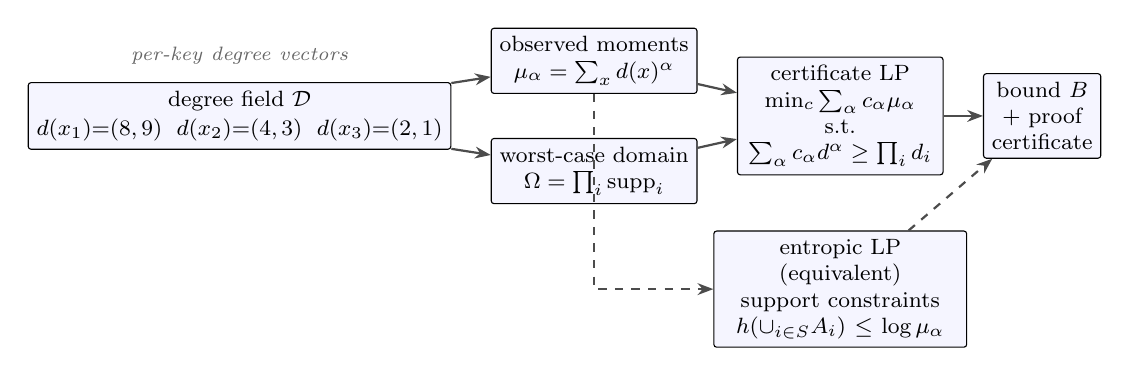
\begin{tikzpicture}[
  font=\footnotesize,
  node distance = 4mm and 5mm,
  box/.style = {draw, rounded corners=1pt, align=center,
                inner sep=3pt, fill=blue!4},
  lab/.style = {font=\scriptsize\itshape, text=black!60},
  arr/.style = {-{Stealth[length=2mm]}, thick, black!70}]

\node[box] (field) {degree field $\mathcal{D}$\\[1pt]
  $d(x_1){=}(8,9)$\; $d(x_2){=}(4,3)$\; $d(x_3){=}(2,1)$};
\node[lab, above=1mm of field] {per-key degree vectors};

\node[box, right=of field, yshift=7mm] (mom) {observed moments\\
  $\mu_\alpha = \sum_x d(x)^\alpha$};
\node[box, right=of field, yshift=-7mm] (omega) {worst-case domain\\
  $\Omega = \prod_i \mathrm{supp}_i$};

\node[box, right=of mom, yshift=-7mm, text width=24mm] (clp)
  {certificate LP\\ $\min_c \sum_\alpha c_\alpha \mu_\alpha$\\
   s.t.\ $\sum_\alpha c_\alpha d^\alpha \ge \prod_i d_i$};

\node[box, right=of clp] (bound) {bound $B$\\ $+$ proof\\certificate};

\node[box, below=7mm of clp, text width=30mm] (elp)
  {entropic LP (equivalent)\\ support constraints
   $h(\cup_{i\in S}A_i) \le \log\mu_\alpha$};

\draw[arr] (field) -- (mom);
\draw[arr] (field) -- (omega);
\draw[arr] (mom) -- (clp);
\draw[arr] (omega) -- (clp);
\draw[arr] (clp) -- (bound);
\draw[arr, dashed] (mom) |- (elp);
\draw[arr, dashed] (elp) -- (bound);
\end{tikzpicture}
\caption{The \framework{} pipeline.  A join induces a degree field on
its separator; statistics are moments of the field; a bound is either
a polynomial certificate over the worst-case domain (top path) or a
support constraint inside the entropic LP (bottom path) --- two views
of the same moment problem.}
\label{fig:pipeline}
\end{figure}

We now re-derive join-size bounds from scratch --- no entropies, no
$h(U)$ variables --- as a moment problem over a combinatorial object
we call the \emph{degree field}.  All prior bounds reappear as
sections of one linear program.

\subsection{The Degree Field and the Product Moment}

\begin{definition}[Degree field]
\label{def:field}
Let $Q$ be a \emph{star query} on separator $X$, i.e., $A_i \cap A_j =
\{X\}$ for $i\neq j$, or more generally a query decomposed at a
separator attribute $X$.  For each key $x \in \mathrm{dom}(X)$ its
\emph{degree vector} is
$d(x) = \big(d_1(x),\dots,d_m(x)\big) \in \mathbf{N}^m$ with
$d_i(x) = \big|\sigma_{X=x}(R_i)\big|$
(the tuple multiplicity, including row multiplicity under bag
semantics).  The multiset $\mathcal{D} = \{d(x)\}_x$ is the
\emph{degree field} of $Q$ at $X$.
\end{definition}

\begin{proposition}[Product moment]
\label{prop:prod}
For a star query on $X$, $|Q| = \sum_x \prod_i d_i(x)$.  For a general
acyclic query with join tree $\mathcal{T}$, $|Q|$ is a product of such
sums over the separators of $\mathcal{T}$.
\end{proposition}

\begin{definition}[Observed moments]
A \emph{statistic} is a moment
$\mu_\alpha = \sum_x d(x)^\alpha$, $\alpha \in \mathbf{N}^m$.
\end{definition}

\noindent Familiar statistics are moments of particular orders:

\begin{center}\small
\begin{tabular}{c|c|l}
$\alpha$ & moment $\mu_\alpha$ & known statistic \\ \hline
$p\cdot e_i$ & $\sum_x d_i(x)^p$ & $\|\deg_i\|_p^p$ \;(all of LpBound) \\
$e_i{+}e_j$ & $\sum_x d_i d_j$ & $|R_i \Join_X R_j|$ \;(pair count) \\
$e_i{+}e_j{+}e_k$ & $\sum_x d_i d_j d_k$ & triple count \\
$\mathbf{0}$ & $\sum_x 1$ & $|\mathrm{dom}(X)|$ \;(support) \\
\end{tabular}
\end{center}

\noindent Note what this view explains immediately: univariate moments
$\{p\,e_i\}$ are \emph{permutation-blind} within each axis --- they
cannot see which $d_i(x)$ pairs with which $d_j(x)$.  The join size is
a \emph{joint} moment; observing it (or any $\alpha$ with $\ge 2$
nonzero coordinates) is precisely the fix.

\subsection{The Certificate LP}

Fix a moment set $\mathcal{A} \subset \mathbf{N}^m$ and let
$\boldsymbol{\mu} = (\mu_\alpha)_{\alpha\in\mathcal{A}}$ be observed
on the realized field.  Since scalar moments do not reveal the
alignment of coordinates, a valid certificate must dominate the
product on the \emph{worst-case domain}
\begin{equation}
\Omega \;=\; \prod_{i=1}^{m} \big( \{0\} \cup \mathrm{supp}(\deg_i)\big)
\;\subseteq\; \mathbf{N}^m .
\label{eq:omega}
\end{equation}

\begin{definition}[Certificate bound]
\label{def:cert}
\begin{align}
UB(\mathcal{A}) &= \min_{c \ge 0}\; \sum_{\alpha\in\mathcal{A}} c_\alpha \mu_\alpha
\quad\text{s.t.}\quad \sum_\alpha c_\alpha d^\alpha \ge \prod_i d_i
\;\;\forall d\in\Omega, \label{eq:ub}\\
LB(\mathcal{A}) &= \max_{c \ge 0}\; \sum_\alpha c_\alpha \mu_\alpha
\quad\text{s.t.}\quad \sum_\alpha c_\alpha d^\alpha \le \prod_i d_i
\;\;\forall d\in\Omega. \label{eq:lb}
\end{align}
\end{definition}

\noindent An upper bound is thus \emph{literally} a nonnegativity
certificate for $\sum_\alpha c_\alpha d^\alpha - \prod_i d_i$ on
$\Omega$: classical inequalities --- AM--GM ($abc \le
\frac{a^3+b^3+c^3}{3}$), Young, H\"older --- are the closed-form
members of this cone; the LP selects the best one \emph{adapted to
the observed $\boldsymbol{\mu}$}.

\begin{theorem}[Duality: bounds are extremal alignments]
\label{thm:dual}
The dual of~\eqref{eq:ub} is the \emph{moment LP}
\[
UB(\mathcal{A}) = \max_{\nu \ge 0 \text{ on } \Omega}\; \sum_y \nu(y)\prod_i y_i
\;\;\text{s.t.}\;\; \sum_y \nu(y)\, y^\alpha = \mu_\alpha \;\forall\alpha ,
\]
i.e., the bound equals the largest product moment over all weightings
(alignments) of $\Omega$ consistent with the observed moments; strong
duality holds since the primal is feasible with finite optimum.
Symmetrically, $LB(\mathcal{A})$ is the \emph{best}-case alignment.
\end{theorem}

\noindent This is the semantic reading of a bound: it answers ``how
large can the join be under the worst alignment of degrees consistent
with the data we measured?''  The certificate $c$ is the dual
proof of that answer.

\begin{example}[A three-key star]
\label{ex:three}
Let $Q = R(X,Y) \Join_X S(X,Z)$ on domain $\{x_1,x_2,x_3\}$ with
degree field $d(x_1) = (8,9)$, $d(x_2) = (4,3)$, $d(x_3) = (2,1)$;
hence $|Q| = 72 + 12 + 2 = 86$.  Univariate moments are
$\mu_{(2,0)} = 84$, $\mu_{(0,2)} = 91$, and
$\Omega = \{8,4,2\}\times\{9,3,1\}$.  Minimizing
$84\,c_{(2,0)} + 91\,c_{(0,2)}$ subject to
$c_{(2,0)}a^2 + c_{(0,2)}b^2 \ge ab$ on the nine grid points gives
the Cauchy certificate $(a^2\,t + b^2/t)/2$ at
$t^\star = \sqrt{91/84}$, i.e.\ $UB = \sqrt{84\cdot91} = 87.45$
--- the conjugate H\"older bound.  Now permute the second coordinate
to $(9,3,1) \mapsto (1,3,9)$: \emph{every} univariate moment is
unchanged, so the bound stays $87.45$ while the true join drops to
$8{+}12{+}18 = 38$.  Adding the level-2 moment
$\mu_{(1,1)} = \langle d_1,d_2\rangle$ separates the two instances:
$c_{(1,1)} = 1$ is a certificate on $\Omega$, giving $UB = \mu_{(1,1)}
= |Q|$ exactly in both cases.
\end{example}

\subsection{The H\"older Section}
\label{sec:holder}

Two facts locate the classical bounds inside the framework.

\begin{proposition}[Univariate moments $=$ H\"older, up to the exponent lattice]
\label{prop:holder}
For $\mathcal{A} = \{p\,e_i : p \in P\}$ the certificate LP plays the
role of the conjugate-H\"older bound
$\min_{\sum_i 1/p_i = 1} \prod_i \|\deg_i\|_{p_i}$, with two
differences: (i) the LP's certificates correspond to conjugates
restricted to the lattice $P$ --- a closed-form scan over
\emph{continuous} conjugates can be tighter when the optimum is
non-integral; (ii) dominance is required only on realized degree
values, not all of $\mathbf{R}^m$ --- so the LP is often strictly
tighter than any closed-form point.
\end{proposition}

\begin{proposition}[The entropy LP implies H\"older on pairs]
\label{prop:implied}
In the entropic LP with atom-wise $q$-inequalities~\eqref{eq:qineq},
every connected pair $i,j$ satisfies~\eqref{eq:holderpair}.
\end{proposition}

\begin{proof}
Write $X = A_i\cap A_j$, $U_i = A_i \setminus X$, $U_j = A_j\setminus
X$.  The $q$-inequalities give
$h(X,U_i) \le (1-\frac1p)h(X) + \log\|\deg_i(U_i|X)\|_p$-style bounds
and symmetrically for $j$ with conjugate $q$; elementary
submodularity on the shared separator gives
$h(A_i\cup A_j) \le h(A_i) + h(A_j) - h(X)$.  Summing cancels the
$h(X)$ coefficients since $(1-\tfrac1p)+(1-\tfrac1q)-1 = 0$, leaving
$\log\|\deg_i\|_p + \log\|\deg_j\|_q$.
\end{proof}

\noindent In words: \emph{the entropic LP's implied bound on each pair
is already the H\"older relaxation of the pair join count}; adding
the exact pair moment pins that relaxation to
$\langle \deg_i,\deg_j\rangle$.  The per-pair quantity
\begin{equation}
\mathrm{gap}_{ij} \;=\; \log \frac{\min_{\text{conj.}}\|\deg_i\|_p\|\deg_j\|_q}
{\langle \deg_i, \deg_j \rangle}
\label{eq:gap}
\end{equation}
is therefore a \emph{computable} predictor of what the level-2 moment
buys over level~1 --- the basis of statistic selection under a
budget.

\subsection{The Hierarchy and Exactness}
\label{sec:hier}

For $\mathcal{A}_k = \{\alpha : |\alpha|_1 \le k\}$ the bounds are
monotone, $UB(1) \ge UB(2) \ge \cdots$ --- a Lasserre-style moment
hierarchy~\cite{lasserre2001} over the field.

\begin{proposition}[Top level is exact]
\label{prop:exact}
If $\mathbf{1} = (1,\dots,1) \in \mathcal{A}$ then
$UB(\mathcal{A}) = |Q|$ on star queries, since $\mu_{\mathbf{1}}$
\emph{is} the product moment.  Hence $m$-atom stars need the $m$-th
moment; on STATS, all $m{=}3$ stars are exact at level~3.
\end{proposition}

Support information in $\Omega$ tightens this further:

\begin{lemma}[Key collapse]
\label{lem:collapse}
If $\mathrm{supp}(\deg_i) \subseteq \{0,1\}$ (a uniqueness constraint
on the separator), then $\alpha = \mathbf{1} - e_i$ is a feasible
monomial certificate and
$UB \le \mu_{\mathbf{1}-e_i} = |Q| +
\sum_{x\in(\cap_{j\ne i}\mathrm{supp}_j)\setminus \mathrm{supp}_i}
\prod_{j\ne i} d_j(x)$.  Exactness at level $m{-}1$ therefore needs
both $d_i \equiv 1$ \emph{and} $\mathrm{supp}_i \supseteq
\cap_{j\ne i}\mathrm{supp}_j$.  On STATS $m{=}4$ stars, all six
exactly-estimated queries carry a $\max\deg{=}1$ atom; on the single
query with a collapsed-but-not-covering atom the bound overshoots by
exactly the predicted uncovered mass.
\end{lemma}

\subsection{The Lower-Bound Wing}
\label{sec:lbwing}

The framework is symmetric: $LB(\mathcal{A})$ of~\eqref{eq:lb} is the
best-case alignment.  Here the polynomial cone honestly fails: on
stars with $m\ge 3$ the best monomial certificate under $\prod d_i$ is
$0$, because the inclusion--exclusion term
$\max(0,\sum_i d_i - (m{-}1))$ is piecewise-linear, not polynomial.
The matching basis is the family of \emph{hinge functions} of the
form $d \mapsto \max(0,\langle w,d\rangle - t)$, whose field
expectations are the
inclusion--exclusion moments; bounds remain one object --- extremal
moments over alignments --- with certificates as conic combinations
of a chosen basis.

\subsection{Scalability: Small LPs and Separation}
\label{sec:sep}

The certificate LP has $|\mathcal{A}|$ variables and $|\Omega|$ rows;
$\Omega$ is exponential only in $m$ (atoms on the separator), not in
the $n$ attributes of the query --- the $2^n$ blow-up of the entropic
LP disappears.  When $|\Omega| = \prod_i |\mathrm{supp}_i|$ is large
we solve~\eqref{eq:ub} by \emph{separation} (cutting planes): solve on
a seed domain, query an oracle for the most-violated grid point, add
it, repeat.  Convergence returns a certificate dominating the
\emph{entire} product --- soundness is proved, not sampled.

\section{\framework{}: Moments in the Entropic LP}
\label{sec:method}

The certificate LP of \S\ref{sec:theory} is the canonical object.  For
\emph{general} queries (cyclic, multi-separator, with group-by
targets) the entropic LP remains the natural host: its variables
interpolate between separators.  We therefore instantiate the moment
hierarchy inside the entropic LP --- each observed joint moment
becomes one support constraint --- while the certificate LP
cross-validates the result on stars (\S\ref{sec:exp}).

\subsection{Pair and Triple Statistics}

\begin{definition}[Moment statistics, entropy side]
\label{def:pairstat}
For every \emph{connected} pair of atoms $i,j$ --- those sharing at
least one attribute --- record the exact join count
$\pcnt_{ij} = |R_i \Join_{A_i\cap A_j} R_j|$ and add
\begin{equation}
h(A_i \cup A_j) \;\le\; \log_2 \pcnt_{ij} .
\label{eq:pair}
\end{equation}
Analogously, for every connected triple, $\tcnt_{ijk} =
|R_i\Join R_j\Join R_k|$ yields $h(A_i\cup A_j\cup A_k) \le
\log_2\tcnt_{ijk}$.
\end{definition}

\begin{theorem}[Soundness]
\label{thm:sound}
For any distribution on the output of $Q$, the marginal on
$A_i\cup A_j$ has support at most $|R_i\Join R_j|$, so
$h(A_i\cup A_j) \le \log_2\pcnt_{ij}$; hence~\eqref{eq:pair} is a
valid inequality of the entropic LP for every database instance.
The same holds for $k$-way counts.
\end{theorem}

\noindent Three properties make this the \emph{right} way to inject a
joint moment:

\begin{itemize}[leftmargin=10pt,itemsep=1pt]
\item \emph{Strongest from one scalar.}  A single number bounds the
  whole joint entropy, including attributes other than the join key.
\item \emph{No new inequality family.}  Unlike
  CorrBound~\cite{mayer2026corrbound} --- which must prove a new
  (conditional-independence) inequality family --- the pair
  constraint is a plain support bound; soundness is Theorem
  \ref{thm:sound}, two lines.
\item \emph{Exact, not sketched.}  We store the exact scalar count
  ($O(1)$ per pair, $O(m^2)$ per query); no sketch error propagates
  into the bound.
\end{itemize}

The count itself is needed only once per pair, at statistics time
(not per query re-optimization), and coincides with the moment
$\mu_{e_i+e_j}$ used by the certificate LP --- the two
representations share one statistic.

\subsection{The Reduced LP}
\label{sec:reduced}

The entropic LP has $2^n$ variables in $n = |V|$ attributes; JOB and
STATS reach $n = 23$.  We keep the solve tractable with the same
reduction as~\cite{zhang2025lpbound}: retain entropic variables only
for a \emph{keepset} (separator attributes and their neighborhoods
needed by active constraints), plus a \emph{ladder} of nested sets
$U \subseteq U \cup \{x\}$ preserving elementary Shannon
inequalities.  On JOB-join the reduced LP reproduces the full-LP
bound bit-for-bit; it shrinks STATS queries from $2^{23}$ to
$O(10^4)$ variables.

\subsection{Proof Certificates}
\label{sec:cert}

Every bound is emitted together with a \emph{certificate}: the dual
variables of the LP, i.e., a conic combination of named constraints
(submodularity, $q$-inequalities, pair supports) that proves
$h(V) \le \log B$.  Checking a certificate needs only linear
arithmetic --- independent of the solver.  This upgrades a bound from
a number to a proof object (in the spirit of
PANDA~\cite{abokhamis2017panda}), and is what let our regression
suite catch four soundness bugs during development
(\S\ref{sec:impl}).

\subsection{Statistics and Implementation}
\label{sec:impl}

\textbf{Counting.}
Pair counts are hash-aggregates $O(|R_i|{+}|R_j|)$; triple counts use
ordered hash joins in $O(\sum|R_i|)$ time with intermediate results
folded into weights, never materialized.  Two SQL-semantics details
are load-bearing: (i) bag semantics --- \texttt{COUNT(*)} counts
\emph{physical rows}, so entropic variables are attached to
duplicate-preserving row identities; (ii) \texttt{NULL}s do not join
--- we encode nulls with per-column unique sentinels so they can
never align, and null-aware predicate comparators keep filtered
degree statistics consistent with SQL three-valued logic.

\textbf{Key identity.}
A join key is a pure value-based function of the tuple, identical
across tables; our regression suite caught a per-table radix-packing
scheme that produced invalid cross-table keys (silently under-counted
pair joins $\Rightarrow$ violated bounds) and a merge-order bug that
dropped an atom reachable only through a later atom in a triple join.
Both surfaced as bound$<$truth violations under certificate
checking --- evidence that the verification pipeline works.

\textbf{Solver.}
LPs are assembled in sparse CSR form; moment columns are
scale-normalized; HiGHS runs with tightened feasibility/optimality
tolerances ($10^{-9}$) plus a presolve/perturbation retry ladder.
For the certificate LP we add a \emph{super-product floor}: any
$\alpha \ge \mathbf{1}$ coordinatewise is itself a valid certificate
($d^\alpha \ge \prod d_i$ on $\mathbf{N}^m$), so $UB$ is capped by
$\min_{\alpha\ge\mathbf{1}}\mu_\alpha$ --- immunizing the reported
bound against numerical sub-optimality of the solver.

\begin{algorithm}[t]
\caption{\framework{} bound computation}
\label{alg:bound}
\begin{algorithmic}[1]
\REQUIRE query $Q$, relations $\{R_i\}$, moment budget $k$
\ENSURE upper bound $B$, proof certificate $\pi$
\STATE collect statistics: $\ell_p$ norms, pair counts $\pcnt_{ij}$,
   $|\alpha|_1 \le k$ counts on connected subsets
\STATE build entropic LP on reduced keepset + ladder (\S\ref{sec:reduced})
\STATE add $q$-inequalities~\eqref{eq:qineq} and support
   constraints~\eqref{eq:pair}
\STATE $h^\star \gets$ LP optimum;\quad $B \gets 2^{h^\star}$
\STATE $\pi \gets$ dual multipliers of binding constraints (\S\ref{sec:cert})
\STATE \RETURN $(B,\pi)$
\end{algorithmic}
\end{algorithm}

\section{Experiments}
\label{sec:exp}

We evaluate \framework{} on the full LpBound evaluation suite plus a
synthetic suite designed to isolate the alignment mechanism.  Three
questions guide the section: \textbf{(Q1)} does observing joint
moments tighten bounds where the theory predicts, and tie where it
predicts a tie? \textbf{(Q2)} does the certificate LP of
\S\ref{sec:theory} reproduce the entropy LP in practice?
\textbf{(Q3)} are all emitted bounds sound?

\textbf{Setup.}  The baseline arm (\emph{lpbound}) is our clean-room
reimplementation of~\cite{zhang2025lpbound}: the entropy LP with all
elementary Shannon inequalities and $q$-inequalities for $p \in
\{1,\dots,10,\infty\}$ over full and simple degree sequences, with
predicates folded into filtered relations before statistics are
computed (stronger than the paper's MCV approximation --- the
baseline gets an unfair advantage).  \emph{+pairs} adds all connected
pair-count constraints~\eqref{eq:pair}; \emph{+triples} adds
connected triples.  Truth is exact \texttt{COUNT(*)} in DuckDB on the
identical parsed rows.  q-error $=$ bound/truth $\ge 1$; any value
$<1$ is a violation.  Solver: HiGHS via scipy; bounds verified
against truth on every evaluated query.

\subsection{Synthetic Mechanism Validation}
\label{sec:exp:syn}

Zipf-distributed degrees on a 3{,}000-key domain; query
$R(X,Y)\Join_X S(X,Z)$ unless noted (Table~\ref{tab:syn}).

\begin{table}[t]
\centering\small
\caption{Synthetic queries (q-err $=$ bound/truth; lower is better)}
\label{tab:syn}
\scalebox{0.92}{
\begin{tabular}{@{}lrrr@{}}
\toprule
case & truth & lpbound & +pairs \\ \midrule
sym (ranks aligned)      & 5.96M & 1.00   & 1.00 \\
\textbf{anti\_rank} (reversed) & 23K & 256.73 & \textbf{1.00} \\
\textbf{anti\_dom} (disjoint)  & 0   & 6.0M   & \textbf{1} \\
asym (skewed supports)   & 27.4M & 1.04   & 1.00 \\
unif                     & 77K   & 1.27   & 1.00 \\
star3/sym                & 9.2B  & 1.00   & 1.00 \\
\textbf{star3/anti\_rank}      & 6.0M  & 1542.72 & \textbf{7.78} \\
j3 chain/correlated      & 2.9M  & 6.49   & 3.86 \\
\textbf{j3 chain/anticorr}     & 29K   & 630.18  & \textbf{206.88} \\
\bottomrule
\end{tabular}}
\end{table}

Three findings.  \emph{(i) Mechanism confirmed}: on two-atom queries
the pair constraint lands on $V$ itself, so every J2 bound is exact
--- including \texttt{anti\_rank} (257$\times$ gap closed) and
\texttt{anti\_dom}, where identical univariate statistics coexist
with a \emph{zero} join.  \emph{(ii) Hierarchy trades storage for
correlation depth}: on the 3-atom star, pairs collapse 1543$\times$
to 7.8$\times$; triples close the rest (Table~\ref{tab:chain}).
\emph{(iii) Residuals are characterized}: the 207$\times$ left on
\texttt{j3/anticorr} is within-relation transitive correlation that
no cross-relation scalar can see --- the predicted limit of level 2.

\begin{table}[t]
\centering\small
\caption{4-chain with one reversed separator (truth $= 42{,}320$)}
\label{tab:chain}
\begin{tabular}{@{}lrr@{}}
\toprule
arm & bound & q-err \\ \midrule
lpbound  & 126{,}823{,}654 & 2996.78 \\
+pairs   & 45{,}071{,}595  & 1065.02 \\
+triples & 7{,}673{,}965   & \textbf{181.33} \\ \bottomrule
\end{tabular}
\end{table}

\textbf{Directed vs.\ undirected graph} (cit-Patents, 3M edges;
Table~\ref{tab:pat}).  On the \emph{directed} graph, in/out-degree
sequences differ and alignment is unobservable: \texttt{p2} goes
4.81$\to$1.00, \texttt{path4} 2067$\to$134 with triples.  On the
\emph{undirected} control, all atoms share one degree sequence, so
$|R_i\Join R_j| = \sum_x \deg(x)^2$ is already implied by the
$p{=}q{=}2$ constraints --- and indeed every bound ties.  This
negative control is the sharp statement of our claim: pair moments
pay off \emph{iff} alignment is not inferable from univariate
marginals.

\begin{table}[t]
\centering\small
\caption{cit-Patents motifs (q-err).  Undirected = negative control.}
\label{tab:pat}
\scalebox{0.92}{
\begin{tabular}{@{}lrrr|rr@{}}
\toprule
& \multicolumn{3}{c|}{directed} & \multicolumn{2}{c}{undirected} \\
motif & lpbound & +pairs & +triples & lpbound & +pairs \\ \midrule
p2     & 4.81    & \textbf{1.00} & ---    & 1.00  & 1.00 \\
tri    & 14.5M   & 3.9M   & ---    & 23.53 & 23.53 \\
claw3  & 1.29    & 1.29   & ---    & 1.26  & 1.26 \\
path3  & 58.95   & 37.84  & ---    & 1.69  & 1.69 \\
path4  & 2067.18 & 2067.18& 133.68 & ---   & --- \\ \bottomrule
\end{tabular}}
\end{table}

\subsection{JOB on IMDB}
\label{sec:exp:job}

The official LpBound workloads: JOB-light (70 queries, 4--8 tables,
predicates), JOB-join (31 queries, up to 14 tables / 23 attributes,
no predicates), JOB-range (1000 queries, range+equality predicates).

\begin{table}[t]
\centering\small
\caption{JOB workloads on IMDB (q-err; viol $=$ bound $<$ truth)}
\label{tab:job}
\scalebox{0.88}{
\begin{tabular}{@{}llrrrrr@{}}
\toprule
workload & arm & geomean & median & p90 & max & exact \\ \midrule
JOB-light & lpbound & 16.14 & 10.12 & 98.0  & 6089   & 0\% \\
(70 q)    & +pairs  & \textbf{4.97} & \textbf{3.89} & \textbf{32.7} & 467 & 6\% \\ \midrule
JOB-join  & lpbound & 10.07 & 4.64  & 123.6 & 4654   & --- \\
(29 q)    & +pairs  & \textbf{5.05} & \textbf{3.46} & \textbf{60.0} & 539 & --- \\ \midrule
JOB-range & lpbound & 111.0 & 90.4  & 2591  & 198533 & 0\% \\
(994 q)   & +pairs  & \textbf{7.30} & \textbf{5.70} & \textbf{67.4} & 13426 & 11\% \\ \bottomrule
\end{tabular}}
\end{table}

Table~\ref{tab:job}: pair moments tighten bounds on 93--100\% of
queries with zero violations.  The largest gain is on JOB-range
(15.2$\times$ geomean), where predicates decorrelate the filtered
degree sequences --- exactly the regime where the H\"older
gap~\eqref{eq:gap} is large.  Highlights: \texttt{jobjoin.27}
4654$\to$540, \texttt{jobjoin.11} 117$\to$6.6; simple stars collapse
to q-err $\approx 1$.

\subsection{STATS on StackOverflow}
\label{sec:exp:stats}

146 queries, heavy predicates, many 4-atom stars (1 truth timeout;
145 evaluated).

\begin{table}[t]
\centering\small
\caption{STATS (145 queries; q-err)}
\label{tab:stats}
\begin{tabular}{@{}lrrrrr@{}}
\toprule
arm & geomean & median & p90 & max & exact \\ \midrule
lpbound  & 175.3 & 108.4 & 14370 & 4.7e8  & 1\% \\
+pairs   & 88.5  & 44.8  & 8710  & 3.1e8  & 8\% \\
+triples & \textbf{8.28} & \textbf{4.91} & \textbf{255} & \textbf{1995} & \textbf{34\%} \\ \bottomrule
\end{tabular}
\end{table}

Triples are the headline (Table~\ref{tab:stats}): a further
10.7$\times$ geomean over pairs, 34\% of queries \emph{exact}.
E.g., \texttt{stats.13} $108\to35\to1.00$, \texttt{stats.14}
$6170\to2240\to1.00$, \texttt{stats.116} $9224\to4002\to22.8$.  The
4-atom stars dominating STATS' tail are the transitive-correlation
regime pairs cannot see; a 3-way marginal covers the connected
skeleton.  Remaining slack (max 1995) is within-relation conditional
correlation --- the motivation for conditional marginals
(\S\ref{sec:conclusion}).

\subsection{DBLP Dense Patterns: Predicted Tie}
\label{sec:exp:dblp}

30 dense 8-vertex subgraph patterns, bound-only protocol (DuckDB
times out on most dense patterns; q-err comparison is on bounds).
Result: \emph{pairs/lpbound bound-ratio geomean $= 1.000$, 100\%
ties}.  Expected: after label propagation each edge atom is tiny
($\sim$9K rows) and the univariate degree sequences already dominate
pair counts --- the same mechanism as the undirected control, now on
real data.

\subsection{Certificate LP = Entropy LP, Verified}
\label{sec:exp:cert}

Solving the certificate LP~\eqref{eq:ub} directly (cutting-plane
separation over $\Omega$) reproduces the entropy LP
\emph{query-by-query} on all 69 single-separator star queries of
STATS: univariate 58.4 vs.\ 58.9 geomean (grid dominance makes the
certificate LP marginally tighter), +pairs 30.6 vs.\ 29.8, +triples
3.73 vs.\ 2.87 (the Shannon web across subset unions captures what
three scalar moments miss on $m{=}4$).  Bit-identical on 17/68
(pair) and 15/63 (triple) cells.  The hierarchy levels are visible
directly: $m{=}3$ stars hit $\mu_{111}{=}$truth on 25/25; $m{=}4$
stars are exact exactly on the six queries carrying a key-collapsed
atom --- Lemma~\ref{lem:collapse} both sufficient and, on this
workload, necessary.

\subsection{Lower Bounds and Intervals}
\label{sec:exp:lb}

The best-case-alignment LP~\eqref{eq:lb} plus spine
inclusion--exclusion emits two-sided intervals: exact (a point) on
every 2-atom query; the interval $[23.1\text{K},\ 5.9\text{M}]$
around truth 28.6K
on \texttt{j3/anticorr}; and $[0,\ 3.9\text{M}]$ certifying possible
emptiness on directed triangles.  On stars with $m\ge3$ the monomial
cone provably degenerates to 0 (\S\ref{sec:lbwing}) --- recorded as
the basis-limitation open problem rather than hidden.

\subsection{Cost and Robustness}
\label{sec:exp:cost}

Storage is one scalar per connected atom subset ($O(m^2)$ pairs).
Statistics are hash aggregates, computed once; JOB-light runs
$\approx$9\,s/query median, dominated by degree-sequence scans on the
33M-row \texttt{cast\_info} --- the reduced LP itself is ms--s.
Regression checking caught four soundness bugs that a synthetic-only
evaluation would have missed (\S\ref{sec:impl}): SQL bag semantics
on row-id attributes, NULL-join semantics, cross-table key packing,
and a merge-order under-count in triple joins.  On badly-scaled
moment LPs, HiGHS can return a numerically suboptimal point; the
super-product floor caps $UB$ at $\min_{\alpha\ge\mathbf{1}}\mu_\alpha$,
and a perturbed-retry ladder recovered 3 of 4 degenerate cells (one
pair cell on \texttt{stats.107} is reported missing rather than
silently looser).

\section{Related Work}
\label{sec:related}

\textbf{Worst-case join size bounds.}
The AGM bound~\cite{atserias2013size,atserias2008agm} introduced the
entropy-counting argument (Shearer's lemma): relation sizes alone give
$|Q| \le \prod_i |R_i|^{w_i}$ over a fractional edge cover.
Worst-case-optimal join algorithms --- NPRR~\cite{ngo2012worst},
Generic Join~\cite{ngo2014skew}, Leapfrog
Triejoin~\cite{veldhuizen2014leapfrog}, Free
Join~\cite{wang2023freejoin} --- attain this bound instance-by-instance.
Degree constraints and PANDA's proof-sequence
algorithm~\cite{abokhamis2017panda} add maximum-degree information and
close the integrality gap on cyclic queries.  Our degree field is the
object these works implicitly bound; we make it explicit and
parameterize bounds by which of its moments are observed.

\textbf{Pessimistic cardinality estimation.}
Cai et al.~\cite{cai2019pessimistic} initiated PCE with size plus
max-degree statistics.  The Degree Sequence
Bound~\cite{deeds2023degree} shows the full sorted degree sequence is
\emph{tight} on Berge-acyclic queries; SafeBound~\cite{deeds2023safebound}
compresses it to segments for practicality.  LpBound~\cite{abokhamis2024lp,
zhang2025lpbound} replaces the sequence by its $\ell_p$-norms inside a
polymatroid LP.  All are univariate in our sense: they bound
\emph{alignment-free} quantities.  \framework{} is a strict extension:
level~1 coincides with LpBound's statistics, and each level $k\ge2$
adds exact $k$-way join counts.

\textbf{Correlation statistics.}
CorrBound~\cite{mayer2026corrbound} is closest: it observes
generalized inner products $\langle a,b\rangle$ of degree vectors and
derives a new information-inequality family, storing sketches and
low-rank factors.  We differ in what is stored (one exact scalar per
connected subset vs.\ sketched vectors), in constraint shape (a direct
support bound $h(A_i\cup A_j) \le \log|R_i\Join R_j|$ vs.\ a new
inequality family), and in verification (exactness means no sketch
error can violate the bound).  Partition
constraints~\cite{deeds2025partition} refine within-relation degree
information by splitting relations; ours is the cross-relation
counterpart.

\textbf{Lower bounds and soundness.}
xBound~\cite{stoian2026xbound} argues for cardinality \emph{lower}
bounds and derives them from reverse inner-product inequalities.  Our
alignment LP gives the lower wing of the same object for free
(\S\ref{sec:lbwing}); identifying its hinge basis as
inclusion--exclusion moments is new.  Provably-correct bounds also
serve as oracle inputs for estimator
validation~\cite{stoian2026outofbounds}.

\textbf{Classical CE.}
Traditional estimators --- histograms, sampling, independence
assumptions --- are unbiased-point-estimate based and notoriously
fragile on joins~\cite{leis2015howgood,leis2018query}; learned
estimators~\cite{han2021cardinality} improve averages but offer no
guarantee.  Pessimistic bounds are complementary: they cap worst-case
error rather than minimize average error.

\textbf{Moment problems.}
Our certificate LP is a truncated generalized moment problem; the
hierarchy parallels Lasserre's SDP/moment
hierarchies~\cite{lasserre2001} in polynomial optimization, with the
combinatorial twist that the domain $\Omega$ is a product of
\emph{discrete} supports and exactness is governed by key-collapse
structure rather than rank conditions.


\section{Conclusion}
\label{sec:conclusion}

We recast join-size bounding as a moment problem on the degree field:
the query answer is a product moment, statistics are observed moments,
and a bound is a polynomial nonnegativity certificate whose dual is a
worst-case alignment.  In this frame, LpBound is the level-1 section
and exact pair/triple join counts are levels 2 and 3 of a Lasserre-style
hierarchy with characterizable exactness conditions.  Instantiated in
the entropic LP, the method improves the state of the art by up to
$21\times$ geomean on the official evaluation suite --- with zero
violations, a predicted negative control on DBLP, and machine-checkable
proof certificates for every number reported.

Three directions remain open.  \emph{Conditional marginals}: the
residual tail on STATS (max 1995$\times$) is within-relation
correlation requiring pair counts conditioned on a third relation's
keys --- a strict generalization of partition constraints across
relations.  \emph{Statistic selection}: the H\"older
gap~\eqref{eq:gap} gives a computable per-pair gain, turning
which-moments-to-materialize into a budgeted optimization problem.
\emph{The lower-bound wing}: hinge bases over inclusion--exclusion
moments complete the two-sided interval picture.  More broadly, the
propose--verify--score loop this paper executes by hand --- propose a
statistic, prove its constraint by a support argument, score it on
bounds --- is a natural target for automation.


\begin{acks}
Kai Wang is the corresponding author.
\end{acks}

%\clearpage

\bibliographystyle{ACM-Reference-Format}
\bibliography{sample}

\end{document}
\endinput
